\documentclass[usenames,dvipsnames,notes,11pt,aspectratio=169,hyperref={colorlinks=true, linkcolor=blue}]{beamer}
\usepackage{ifthen}
\usepackage{xcolor}
\usepackage{pgfplots}
\usepackage{amsmath}
\usepackage{centernot}
\usepackage{pifont}
\usepackage{tabularx}
\usepackage{makecell}
\usepackage{cuted}
\usepackage{booktabs}
\usepackage{array}
\usepackage{textcomp}
\usepackage{setspace}
\usepackage{xspace}
\usepackage{subcaption}
\usepackage{tikz}
\usepackage{pdfcomment}
%\newcommand{\pdfnote}[1]{\marginnote{\pdfcomment[icon=note]{#1}}}
\newcommand{\pdfnote}[1]{}

\usepackage{pgfpages}
%\setbeameroption{show notes on second screen}


\input ../beamer-style
\input ../std-macros
\input ../macros

\newcommand{\pt}{\partial}

\AtBeginSection[]
{
    \begin{frame}
        \frametitle{Table of Contents}
        \tableofcontents[currentsection]
    \end{frame}
}
\parskip=10pt

\title[DS-GA.1011]{Efficient Pretraining and Finetuning Techniques}
\author[He He]{He He
}
\institute[NYU]{
    
\includegraphics[height=1cm]{../figures/nyu-logo}\\
}
\date{October 18, 2023}

\begin{document}
\begin{frame}
\titlepage
\end{frame}

\begin{frame}
    {Logistics}
    \begin{itemize}
        \item HW3 released: finetuning BERT! Due on Nov 3.
    \end{itemize}
\end{frame}

\begin{frame}
    {Introduction}

    Plan for today:\\
    \begin{itemize}
        \item How to train larger models on larger data with less compute
        \item How to finetune larger models with less compute
        \item Goal is to get an overview of the field
    \end{itemize}

    \pause
    Why care about efficiency?\\
    \begin{itemize}
        \item Practical reasons: training and running these models are expensive!
        \item Methods that help scaling may eventually leads to \textit{better} models (e.g., transformers)
            \begin{itemize}
                \item[] {\small\it
                        ``The bitter lesson is based on the historical observations that 1) AI researchers have often tried to build knowledge into their agents, 2) this always helps in the short term, and is personally satisfying to the researcher, but 3) in the long run it plateaus and even inhibits further progress, and 4) breakthrough progress eventually arrives by an opposing approach based on scaling computation by search and learning.'' %The eventual success is tinged with bitterness, and often incompletely digested, because it is success over a favored, human-centric approach.''
                    } --- Richard Sutton ``The bitter lesson''
            \end{itemize}
    \end{itemize}
\end{frame}

\section{Efficient pretraining}

\begin{frame}
    {Overview}
    Approaches to speed up pretraining \pause
    \begin{itemize}
        \itemsep1em
        \item Reduce model size
        \item Design more sample-efficient learning objectives
        \item Improve efficiency of self-attention
        \item Improve system-level efficiency
    \end{itemize}
\end{frame}

\begin{frame}
    {Approach 1: Reduce model size}

    Idea 1: reduce the number of parameters

    ALBERT (a lite BERT) \mycite[https://arxiv.org/abs/1909.11942]{[Lan et al., 2020]}

    \begin{itemize}
            \only<1>{
        \item \textbf{Factorization}:
    \begin{itemize}
        \item Recall that in Transformer, we first need to map the one-hot encoding (of size $\red{V}$) of a token to Q, K, V embeddings (of size $\blue{H}$)
        \item The number of parameters is $\red{V}\times \blue{H}$
        \item We can instead first map it to a lower-dim space (of size $\green{E}$) so that the number of params is $\red{V}\times\green{E} + \green{E}\times\blue{H}$
    \end{itemize}
}
            \only<2->{
\item \textbf{Parameter sharing}:
    \begin{itemize}
        \item Share feedforward network weights across layers
        \item Share self-attention weights across layers
        \item ALBERT: share all params across layers
    \end{itemize}
}
    \end{itemize}
\end{frame}

\begin{frame}
    {Approach 1: Reduce model size}

    Idea 2: reduce interaction among parameters (sparse/modular architectures)

    DEMix \mycite[https://aclanthology.org/2022.naacl-main.407.pdf]{[Gururangan et al., 2022]}

    \begin{columns}
        \begin{column}{0.4\textwidth}
            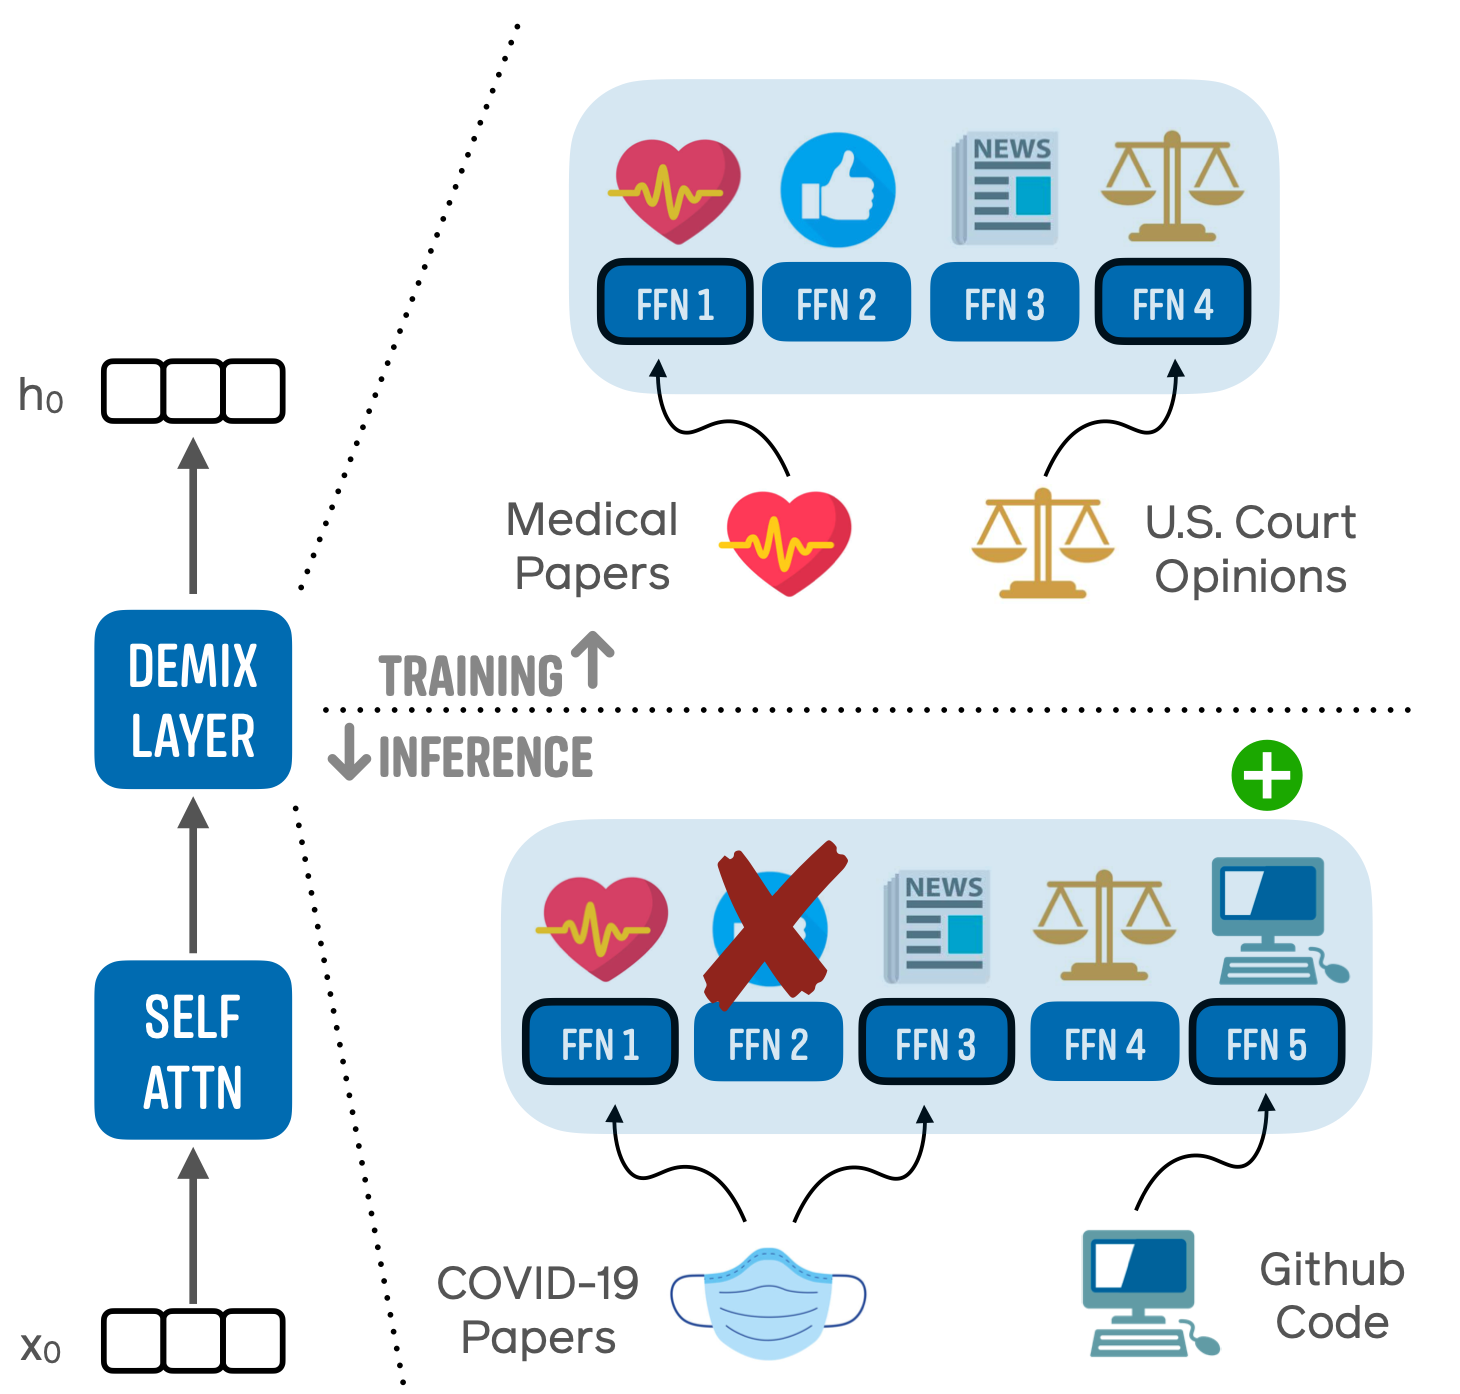
\includegraphics[height=0.6\textheight]{figures/demix}
        \end{column}
        \begin{column}{0.6\textwidth}
            \begin{itemize}
                \item Replace the FFN layer with an ensemble of $n$ experts
                \item Route examples to experts corresponding to its domain determinstically
                    $$
                    \mathrm{FFN}(h) = \sum_{i=1}^n \1{[x \in \text{domain $i$}]} \mathrm{FFN}_i(x)
                    $$
                \item Only a subset of params are active for each example/batch
            \end{itemize}
        \end{column}
    \end{columns}
\end{frame}

\begin{frame}
    {Approach 1: Reduce model size}

    Idea 2: reduce interaction among parameters (sparse/modular architectures)

    Branch-Train-Merge \mycite[https://arxiv.org/pdf/2208.03306.pdf]{[Li et al., 2022]}
    \begin{figure}
            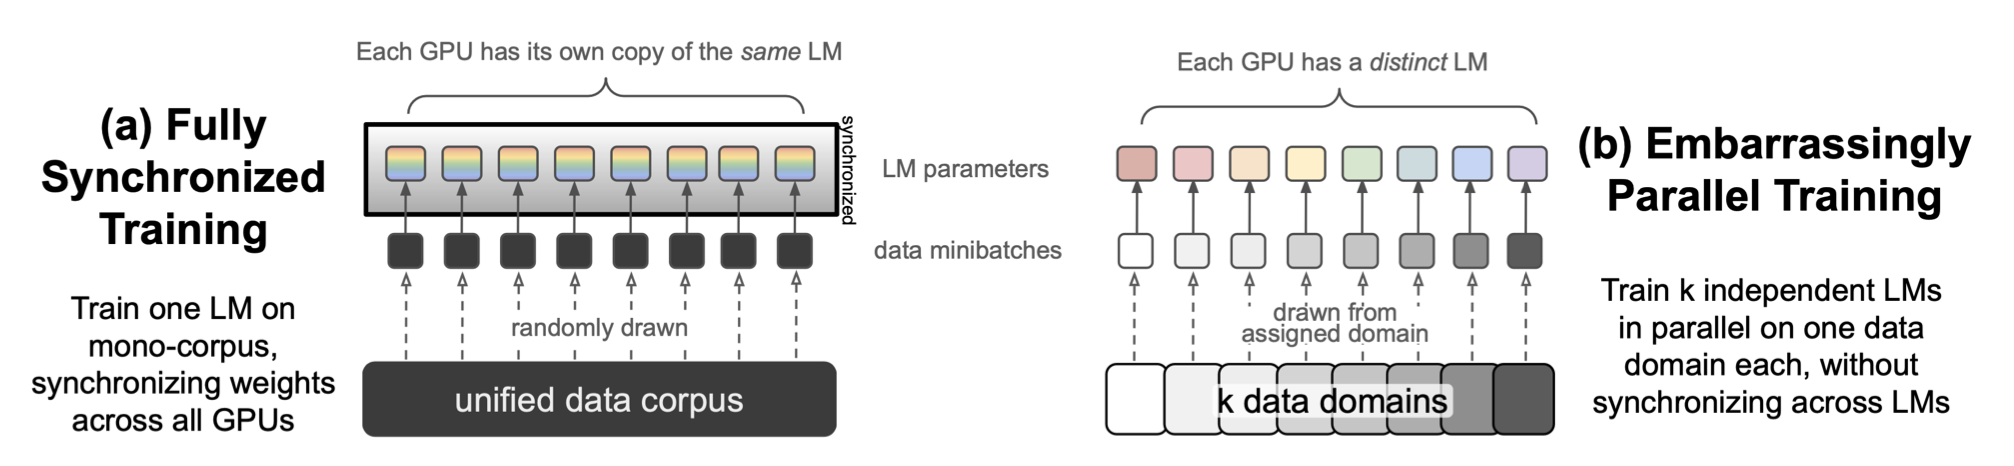
\includegraphics[width=\textwidth]{figures/btm}
    \end{figure}
    \begin{itemize}
        \item Train domain experts in parallel and ensemble them (or take weighted average of their parameters)
        \item Reduce synchronization among GPUs at the cost of increased model size
        \item Easy to expand/remove domain experts 
    \end{itemize}
\end{frame}

\begin{frame}
    {Approach 2: design sample-efficient learning objectives}

    ALBERT: Inter-sentence coherence loss\\
    \begin{itemize}
        \item Motivation: the next sentence prediction task is too easy
        \item Design \blue{hard negative examples}
        \item Input: take two consecutive sentences, swap their order randomly
        \item Output: predict if they are in natural order\\
            \begin{tabular}{ll}
                \textit{I went home. \texttt{SEP} I slept.} & +1\\
                \textit{I slept. \texttt{SEP} I went home.} & -1\\
            \end{tabular}
            
        \item Model needs to learn temporal order of events (commonsense, causality etc.) 
    \end{itemize}
\end{frame}

\begin{frame}
    {Approach 2: design sample-efficient learning objectives}

    ELECTRA \mycite[https://arxiv.org/abs/2003.10555]{[Clark et al., 2020]}: discriminate from true vs guessed tokens

    \vspace{-1em}
    \begin{figure}
        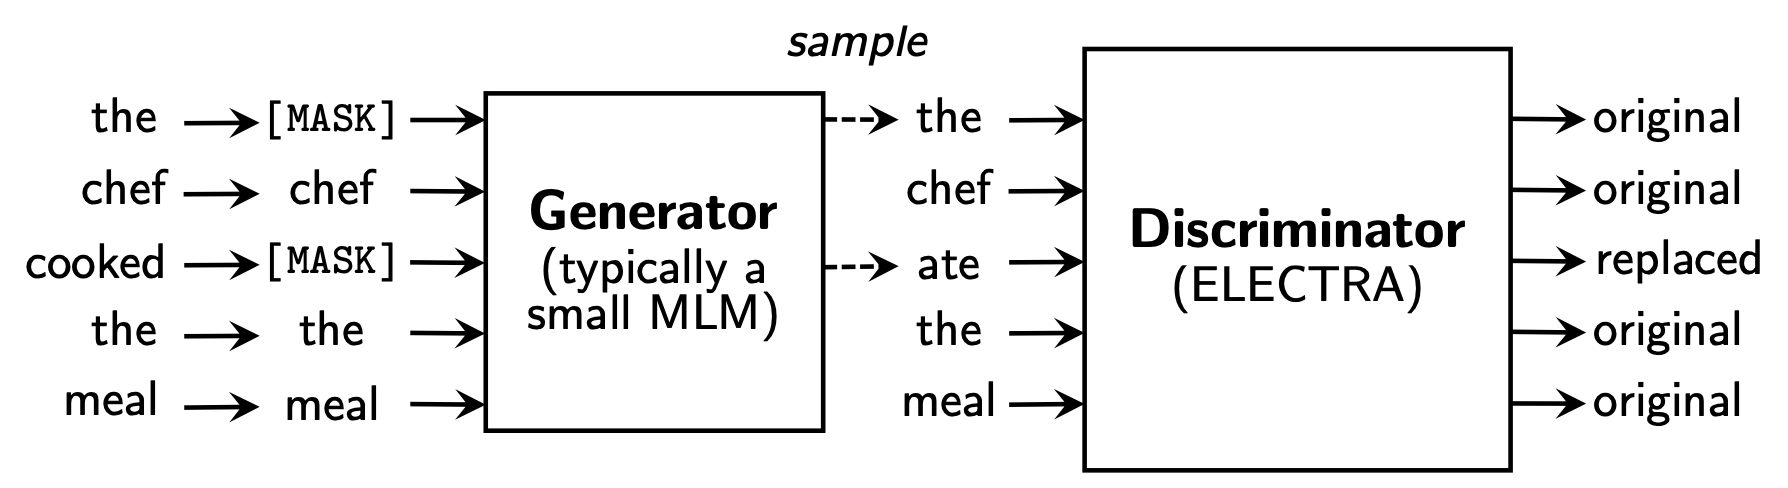
\includegraphics[height=3cm]{figures/electra}
    \end{figure}
    \vspace{-1em}

    \begin{itemize}
        \item First train the generator for n steps using the MLM objective.
        \item Freeze generator weights. Train the discriminator using the sequence classification objective. Keep discriminator for finetuning.
        \item Comparison with MLM: predict at every position; hard negative examples. 
    \end{itemize}
\end{frame}

\begin{frame}
    {Approach 2: design sample-efficient learning objectives}

    ELECTRA result:
    \begin{figure}
        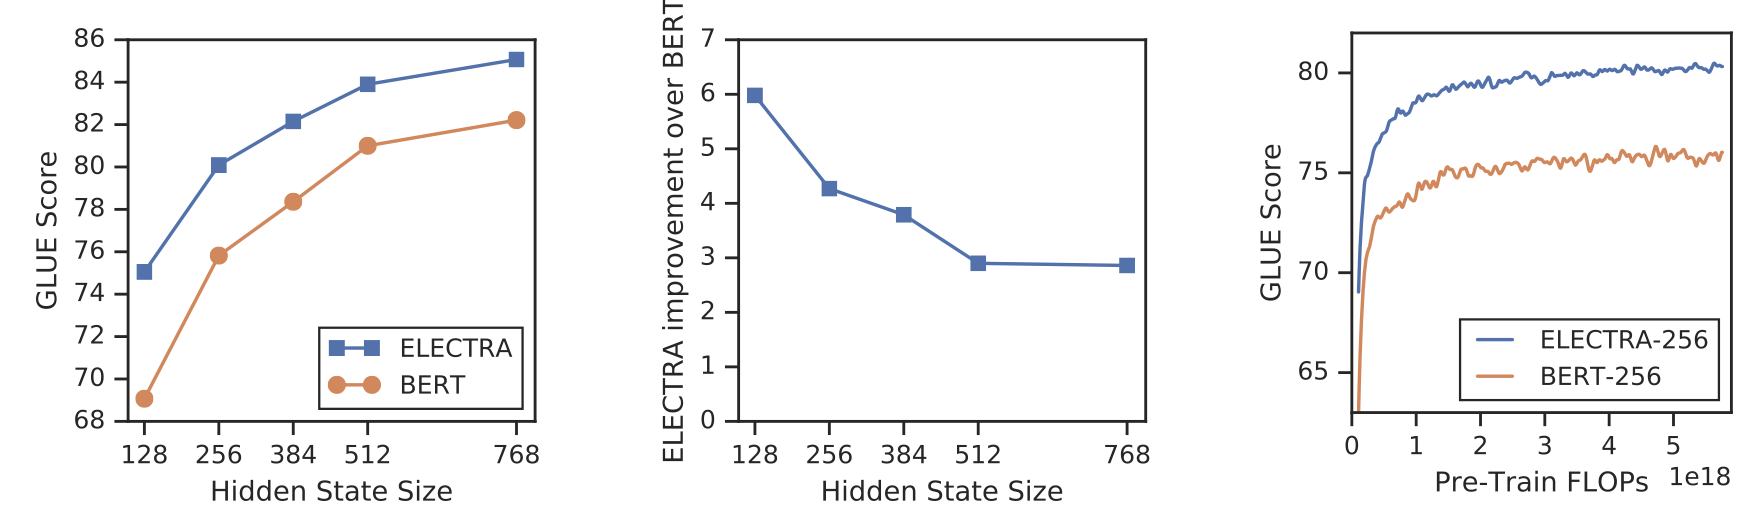
\includegraphics[height=3cm]{figures/electra-result}
        \caption{Finetuning result on the GLUE benchmark}
    \end{figure}
    \begin{itemize}
        \item Larger improvement at smaller model sizes
        \item Faster training 
        \item An effective approach if you don't have large compute for pretraining
    \end{itemize}
\end{frame}

\begin{frame}
    {Approach 3: alternatives to self-attention}

    Transformer recap
    \begin{columns}
        \begin{column}{0.4\textwidth}
    \begin{figure}
        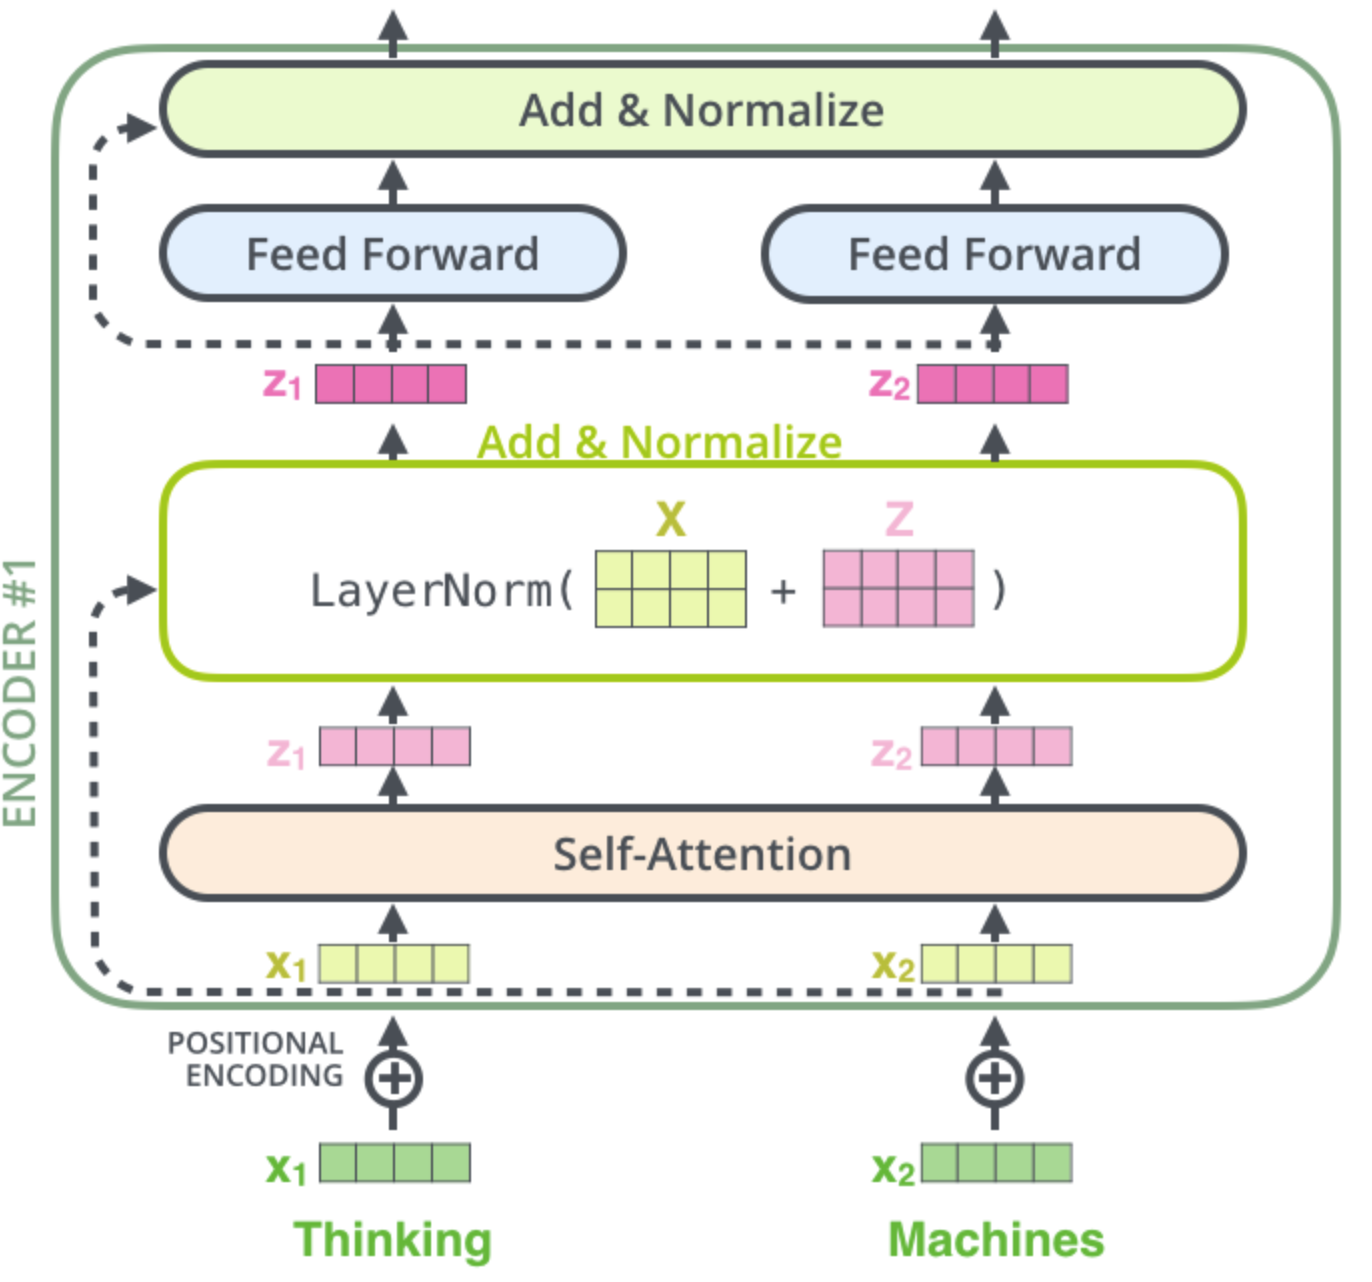
\includegraphics[width=\textwidth]{figures/transformer-block}
        \caption{From \href{https://jalammar.github.io/illustrated-transformer}{The Illustrated Transformer}}
    \end{figure}
        \end{column}
        \begin{column}{0.6\textwidth}
            Which components require matrix multiplication?\\
            \pause
            \begin{itemize}
                \item Self-attention 
                    \begin{itemize}
                        \item Q,K,V projection
                        \item Scaled dot-product attention
                    \end{itemize}
                \item Feed-forward layer
            \end{itemize}
        \end{column}
    \end{columns}
\end{frame}

\begin{frame}
    {Compute cost of transformers}
    Q, K, V projection:\\[1ex]
    \begin{tikzpicture}
        \draw (0,0) rectangle (2, 1) node[pos=.5] {$n\times d_e$};
        \draw (4, 0) rectangle (4+3, 1) node[pos=.5] {$n\times d$};
        \draw[arrow] (2.5, 0.5) -- (3.5, 0.5) node[midway, above] {linear};
        \onslide<2->{
            \node at(4+3+2, 0.5) {$O(n\times d_e \times d)$};
        }
    \end{tikzpicture}

    \medskip\onslide<+->{
    Scaled dot-product attention:\\[1ex]
    \begin{tikzpicture}
        \draw (0,0) rectangle (3, 1) node[pos=.5] {$n\times d$};
        \draw (4, 0) rectangle (4+1, 3) node[pos=.5] {$d\times n$};
        \draw (4+1+2, 0) rectangle (4+1+2+1, 1) node[pos=.5] {$n\times n$};
        \draw[arrow] (4+1+0.5, 0.5) -- (4+1+2-0.5, 0.5) node[midway, above] {matmul};
        \onslide<+->{
            \node at(4+1+2+1+2, 0.5) {$O(d\times n^2)$};}
    \end{tikzpicture}
    }
\end{frame}

\begin{frame}
    {Compute cost of transformers}

    Feed-forward layer (GPT-2):\\[1ex]
    \begin{tikzpicture}
        \draw (0,0) rectangle (2, 1) node[pos=.5] {$n\times d$};
        \draw (4+1, 0) rectangle (4+3+1, 1) node[pos=.5] {$n\times d_h$};
        \draw[arrow] (2.5, 0.5) -- (4+1-0.5, 0.5) node[midway, above] {linear+ReLU};
        \onslide<2->{
        \draw (4+3+1+3, 0) rectangle (4+3+1+3+2, 1) node[pos=.5] {$n\times d$};
        \draw[arrow] (4+3+1+0.5, 0.5) -- (4+3+1+3-0.5, 0.5) node[midway, above] {linear+ReLU};}
    \onslide<.->{
        \node at(0, -1) {$O(n\times d\times d_h)$};
    }
    \end{tikzpicture}

    \onslide<+->{
    \begin{itemize}
        \item Two-layer FFN
        \item $d_h=4d$ ($d>1K$) by default in GPT-2
        \item Approximately half of the compute time
    \end{itemize}
    }
\end{frame}

%\begin{frame}
%    {Improve efficiency of transformers}
%    How to scale transformer models to larger number of parameters and larger data?
%
%    \begin{itemize}
%        \item Quantization (training and inference)
%        \item Weight sharing (training and inference)
%        \item Sparsely-activated models (training and inference)
%        \item Pruning (inference)
%        \item Distillation (inference)
%    \end{itemize}
%\end{frame}

\begin{frame}
    {Improve efficiency of self-attention (for long sequences)}

    \onslide<2->{
    \textbf{Key idea}: reduce the $O(n^2)$ time and memory cost\\
    \begin{itemize}
        \item Sparsify the attention matrix
            % TODO: draw a figure to show the masking
            \begin{itemize}
                \item Deterministic mask
                \item Data-dependent mask (Reformer \mycite[https://arxiv.org/pdf/2001.04451.pdf]{[Kitaev et al., 2020]})
            \end{itemize}
        \item Compress the key-value memory
            % TODO: draw a figure to show the size change 
            \begin{itemize}
                \item Low-rank projection 
                \item Attention-based projection 
            \end{itemize}
    \end{itemize}
    }

\end{frame}

%\begin{frame}
%    {Limiting receptive field of self-attention}
%    \textbf{Blockwise self-attention} \href{https://arxiv.org/pdf/1911.02972.pdf}{[Qiu et al., 2020]}: attention within a local window \\[1em]
%
%    \begin{columns}
%        \begin{column}{0.4\textwidth}
%        {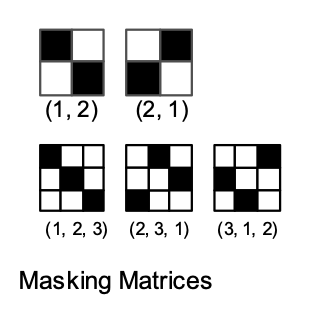
\includegraphics[width=\textwidth]{figures/block-transformer}}
%        \end{column}
%        \begin{column}{0.6\textwidth}
%            \begin{itemize}
%                \item Divide a $n\times n$ matrix into $m\times m$ blocks
%                \item Compute one block per row and mask the rest (i.e. set to 0)
%                \item Allocate groups of attention heads to each mask configuration
%                    \begin{itemize}
%                        \item Which configuration should use more attention heads?
%                    \end{itemize}
%                \pause
%                \item What's the time complexity?\pause
%                    \begin{itemize}
%                        \item $O(n^2) \longrightarrow \red{O(n^2/m)}$ 
%                            \pdfnote{$(n/m)^2 \times m$}
%                    \end{itemize}
%
%            \end{itemize}
%        \end{column}
%    \end{columns}
%\end{frame}

\begin{frame}
    {Sparse attention}
    \textbf{Longformer} \mycite[https://arxiv.org/pdf/2004.05150.pdf]{[Beltagy et al., 2020]}: attention within a local window\\[1ex]

        {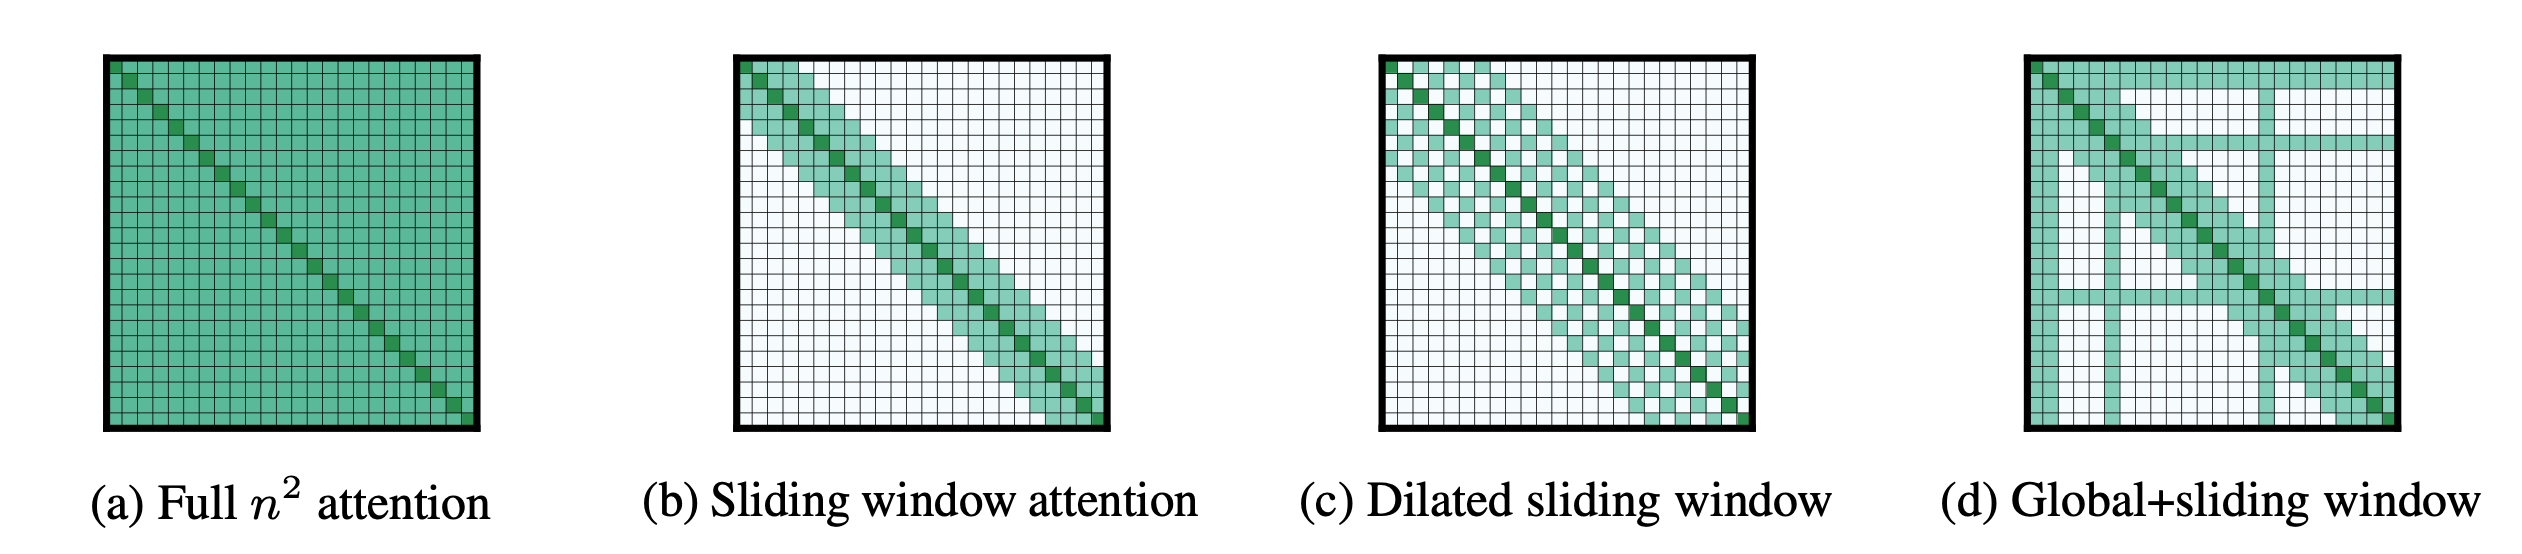
\includegraphics[width=0.8\textwidth]{figures/longformer}}

    \begin{itemize}
        \item \blue{Sliding window}: attending to a \textit{local} window of size $w$ around each token $\red{O(n\times w)}$
        \item \blue{Dilated sliding window}: reaching \textit{longer range} with a larger window size with gaps
        \item \blue{Global window}: \textit{full attention} on specific tokens, e.g., \texttt{[CLS]} in BERT
            \pause
        \item Details: balancing efficiency and performance
            \begin{itemize}
                \item Adding dilation on some heads
                \item Using small window size on lower layers and larger ones on higher layers
            \end{itemize}
    \end{itemize}
\end{frame}

%\begin{frame}
%    {Limiting receptive field of self-attention}
%    \textbf{Reformer} \href{https://arxiv.org/pdf/2001.04451.pdf}{[Kitaev et al., 2020]}: attention within an \blue{adaptive} local window\\[1ex]
%
%    \textbf{Key idea}:\\
%    \begin{itemize}[<+->]
%        \item We want to compute the attention scores for a query $q_i$:
%            $$
%            a_i = \mathrm{softmax}\p{\pb{\frac{q_i\cdot k_1}{\sqrt{d}},\ldots,\frac{q_i\cdot k_n}{\sqrt{d}}}}
%            $$
%        \item \textbf{Goal}: can we approximate $a_i \in \BR^n$ by computing $<n$ dot products?
%        \item Which dot products ($k_j$'s) have large influence on the value $a_i$?
%            \begin{itemize}
%                \item $k_j$'s that has large dot products with (``close to'') $q_i$
%            \end{itemize}
%        \item How do we find such $k_j$'s (\blue{nearest neighbors} of $q_i$) fast?
%            \begin{itemize}
%                \item \textbf{Locality sensitive hashing} (LSH): close vectors are put in the same bucket: $h(k_s) = h(k_t)$ if $k_s$ is close to $k_t$
%            \end{itemize}
%        \item Compute attention between $q_i$ and $k_i$ only if they fall in the same hash bucket
%    \end{itemize}
%\end{frame}
%
%\begin{frame}
%    {Limiting receptive field of self-attention}
%    \textbf{Reformer} \href{https://arxiv.org/pdf/2001.04451.pdf}{[Kitaev et al., 2020]} implementation\\[1em]
%
%    \begin{columns}
%        \begin{column}{0.4\textwidth}
%        {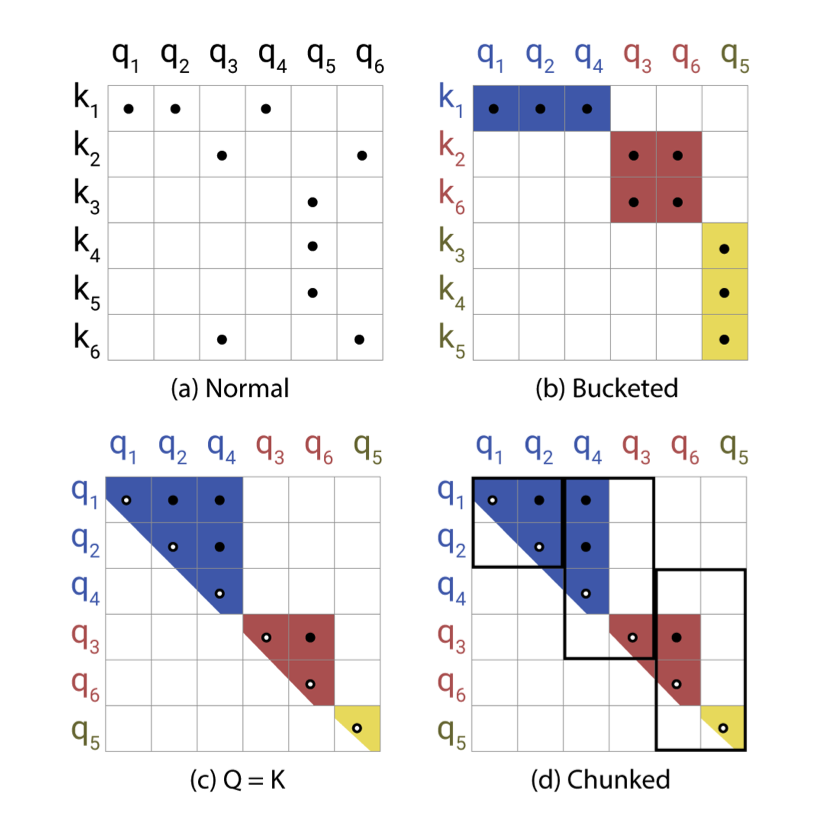
\includegraphics[width=\textwidth]{figures/reformer}}
%        \end{column}
%        \begin{column}{0.6\textwidth}
%            \begin{itemize}[<+->]
%                \item[(a)] Leverage the sparsity of the attention matrix
%            \end{itemize}
%
%            \onslide<+->{
%            \textbf{Challenge 1}: find the nearest neighbors\\
%            \begin{itemize}[<+->]
%                \item[(b)] Sort $q_i$'s and $k_i$'s by their hash codes such that \blue{vectors in the same bucket} are grouped %\hfill \textit{\red{uneven in size}}
%            \end{itemize}
%            }
%
%            \onslide<+->{
%            \textbf{Challenge 2}: batch the computation\\
%            \begin{itemize}[<+->]
%                \item[(c)] Set $k_i = q_i$ such that similar vectors are grouped along the diagonal 
%                \item[(d)] Chunk it by \blue{equal size} (cf. blockwise attention)  \hfill\textit{\red{a group may be split in two chunks}}
%                    \begin{itemize}
%                        \item Each chunk attends to itself and the previous chunk 
%                    \end{itemize}
%            \end{itemize}
%            }
%
%            \onslide<+->{
%                \textit{Better accuracy with more hashes}}
%        \end{column}
%    \end{columns}
%\end{frame}

\begin{frame}
    {Compresse the KV memory}

    Self-attention is low rank \href{https://arxiv.org/pdf/2006.04768.pdf}{[Wang et al., 2020]}\\[1ex]
    {\centering
    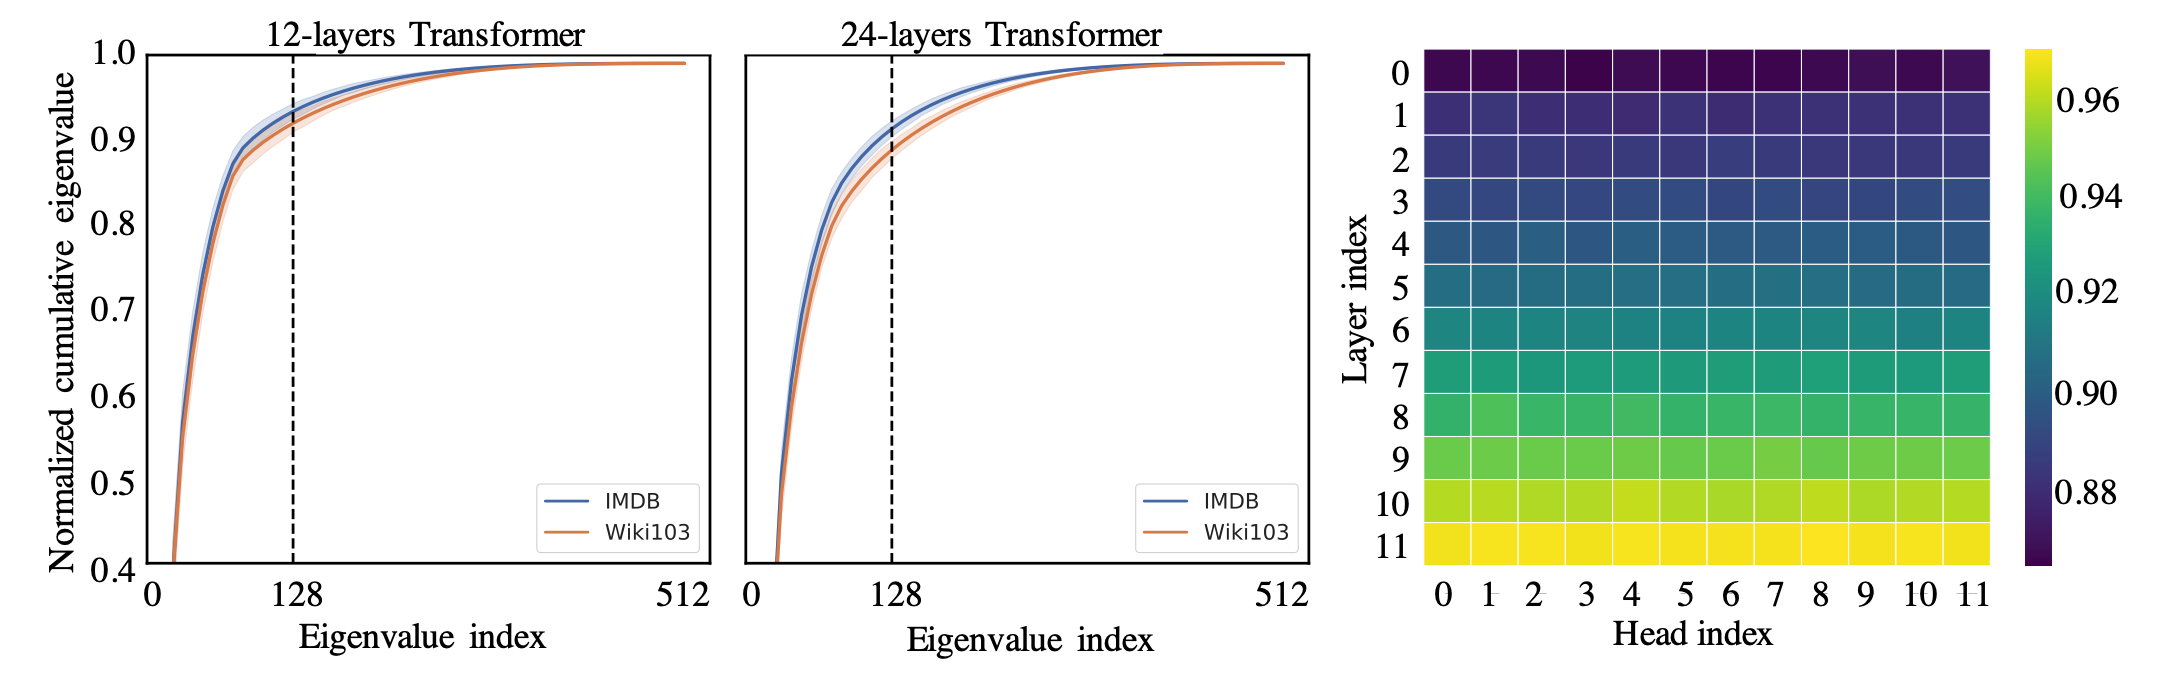
\includegraphics[height=3cm]{figures/low-rank}}

    \begin{itemize}[<+->]
        \item Left: cumulative eigenvalues of pretrained transformer with $n=512$
            \begin{itemize}
                \item Most information in the attention matrix can be recovered by the top 128 eigenvectors %explains $>90\%$ of the variance
            \end{itemize}
        \item Right: cumulative eigenvalues of the top 128 eigenvalues across layers 
            \begin{itemize}
                \item Higher layers are more low-rank 
            \end{itemize}
        \item \textbf{Idea}: instead of attending to $n$ tokens, attend to $k$ principal components 
    \end{itemize}
\end{frame}

\begin{frame}
    {Summarize the KV memory}

    \textbf{Linformer} \mycite[https://arxiv.org/pdf/2006.04768.pdf]{[Wang et al., 2020]}: compute self-attention in a lower dimension \\[1em]

    \begin{columns}
        \begin{column}{0.3\textwidth}
        {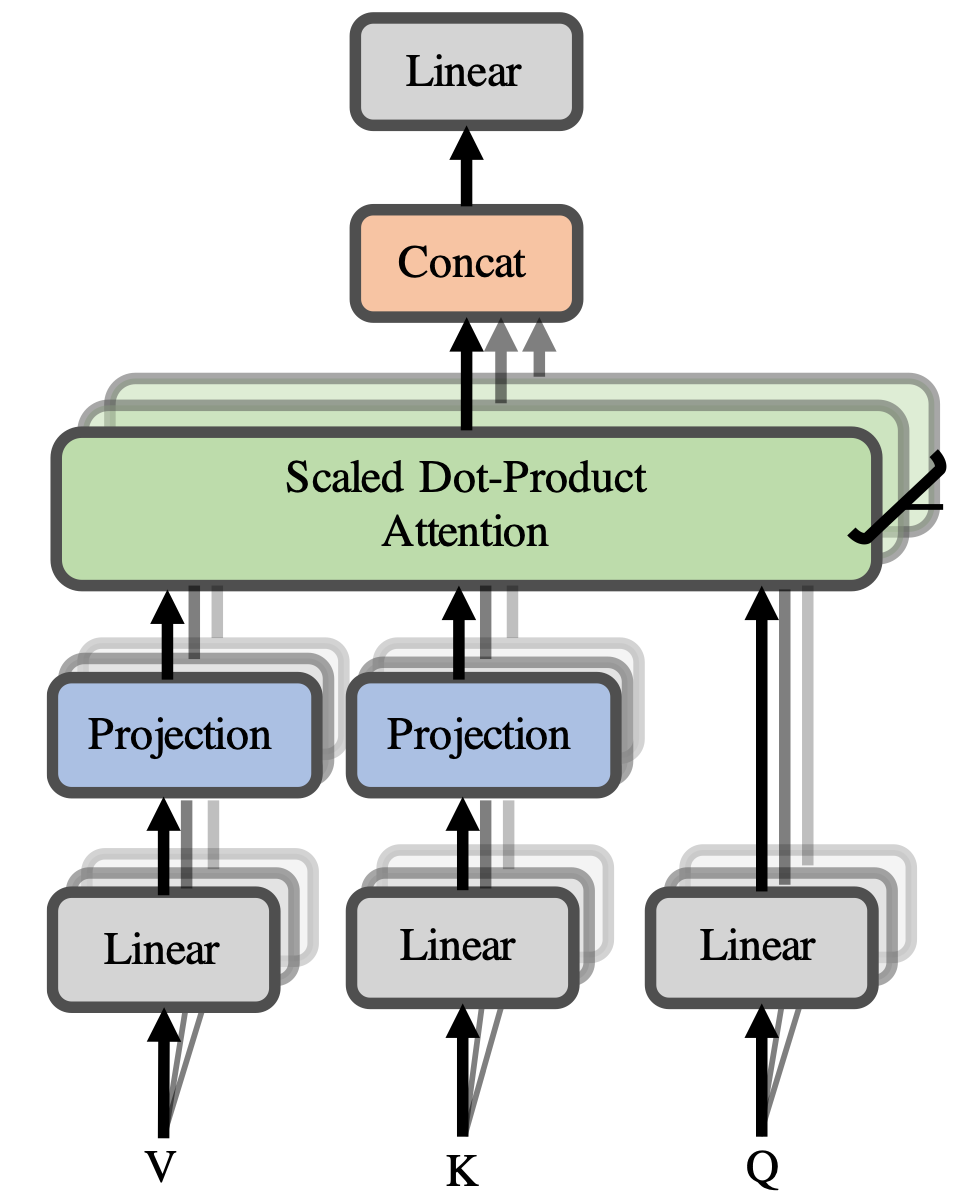
\includegraphics[width=\textwidth]{figures/linformer}}
        \end{column}
        \begin{column}{0.7\textwidth}
            \begin{itemize}[<+->]
                \item Reduce dimensionality of the ``memory'': Map K, V from $n\times d$ to $\blue{k}\times d$
                \item Attend to the lower-dimensional memory: $\mathrm{softmax}\p{Q_{n\times d}K^T_{k\times d}/\sqrt{d}}$
                    \begin{itemize}
                        \item What's the dimension of the attention matrix?
                            \pdfnote{n x k}
                        \item What's the dimension of the self-attention output?
                            \pdfnote{n x d}
                    \end{itemize}
                \item Computation cost: \red{$O(nk)$} (linear in $n$)
                \item Downside of uisng Linformer as a decoder?
                    \begin{itemize}
                        \item Unclear how to mask: past and future are mixed
                    \end{itemize}
            \end{itemize}
        \end{column}
    \end{columns}
\end{frame}

\begin{frame}
    {Compress the KV memory}
    \textbf{Perceiver} \href{https://arxiv.org/pdf/2103.03206.pdf}{[Jaegle et al., 2021]}: use latent states to compress the KV memory \\[1em]

    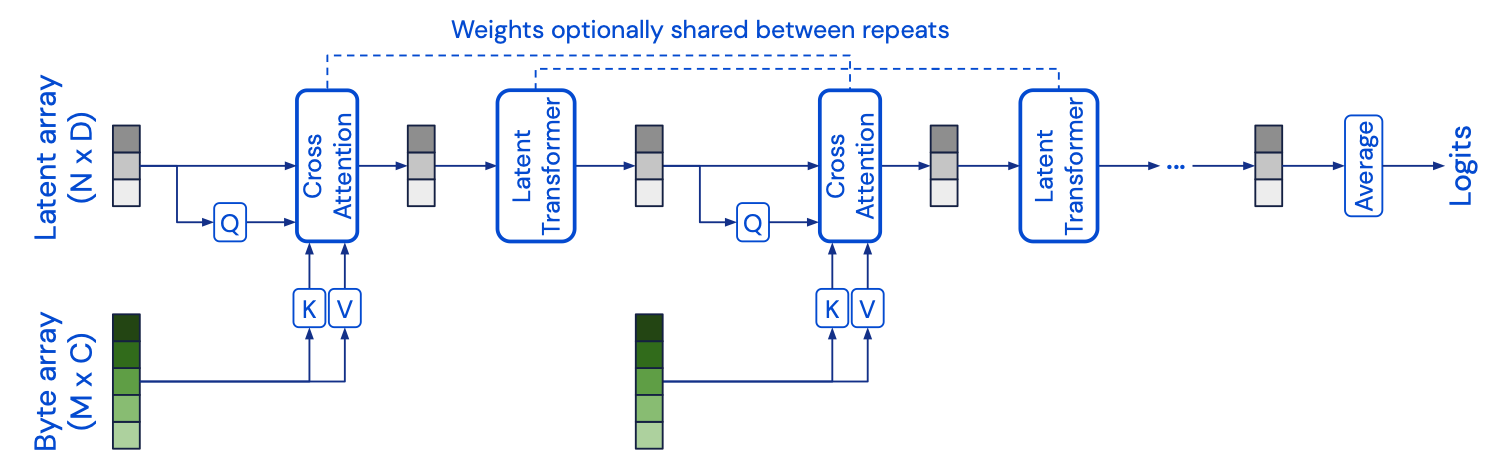
\includegraphics[height=3.5cm]{figures/perceiver}

    \begin{itemize}[<+->]
        \item Use latent states ($k\times d_s$) as queries to attend to K,V ($n\times d$) $\longrightarrow$ compress KV memory to lower dimensional states ($k\times d_s$)
        \item Map to latent states using cross attention: \red{$O(nk)$}
        \item Self-attention layers on lower dimenstional \textit{latent states} ($O(k^2)$)
    \end{itemize}
\end{frame}

%\begin{frame}
%    {Mixture-of-experts models}
%\end{frame}

\begin{frame}
    {Summary on efficient self-attention}

    Improve the quadratic time and space complexity of self-attention\\
    \begin{itemize}
        \item Sparsify the attention matrix
        \item Compress the KV memory
    \end{itemize}

    \pause
    Bad news: Most techniques are not widely used in large pretrained models now. Why?\\
    \begin{itemize}
        \item Improvement in time/space complexity doesn't always translate to real time/space savings
        \item These techniques often breaks structure and sacrifice the batching ability on GPUs
        \item Only see improvement on very long sequences
    \end{itemize}
    %\pause
    %Takeaways:\\
    %\begin{itemize}
    %    \item Attention structure is important
    %    \item Low-rank techniques
    %\end{itemize}
\end{frame}

\begin{frame}
    {Approach 4: system-level approaches}
    \begin{itemize}
        \item Operates at a lower abstraction level
        \item Often brings more direct impact on efficiency
        \item Example:
            \begin{itemize}
                \item Gradient accumulation
                \item Model and data parallelism (e.g., deepspeed)
                \item Flash attention: exploit GPU memory asymmetry
                    \begin{figure}
    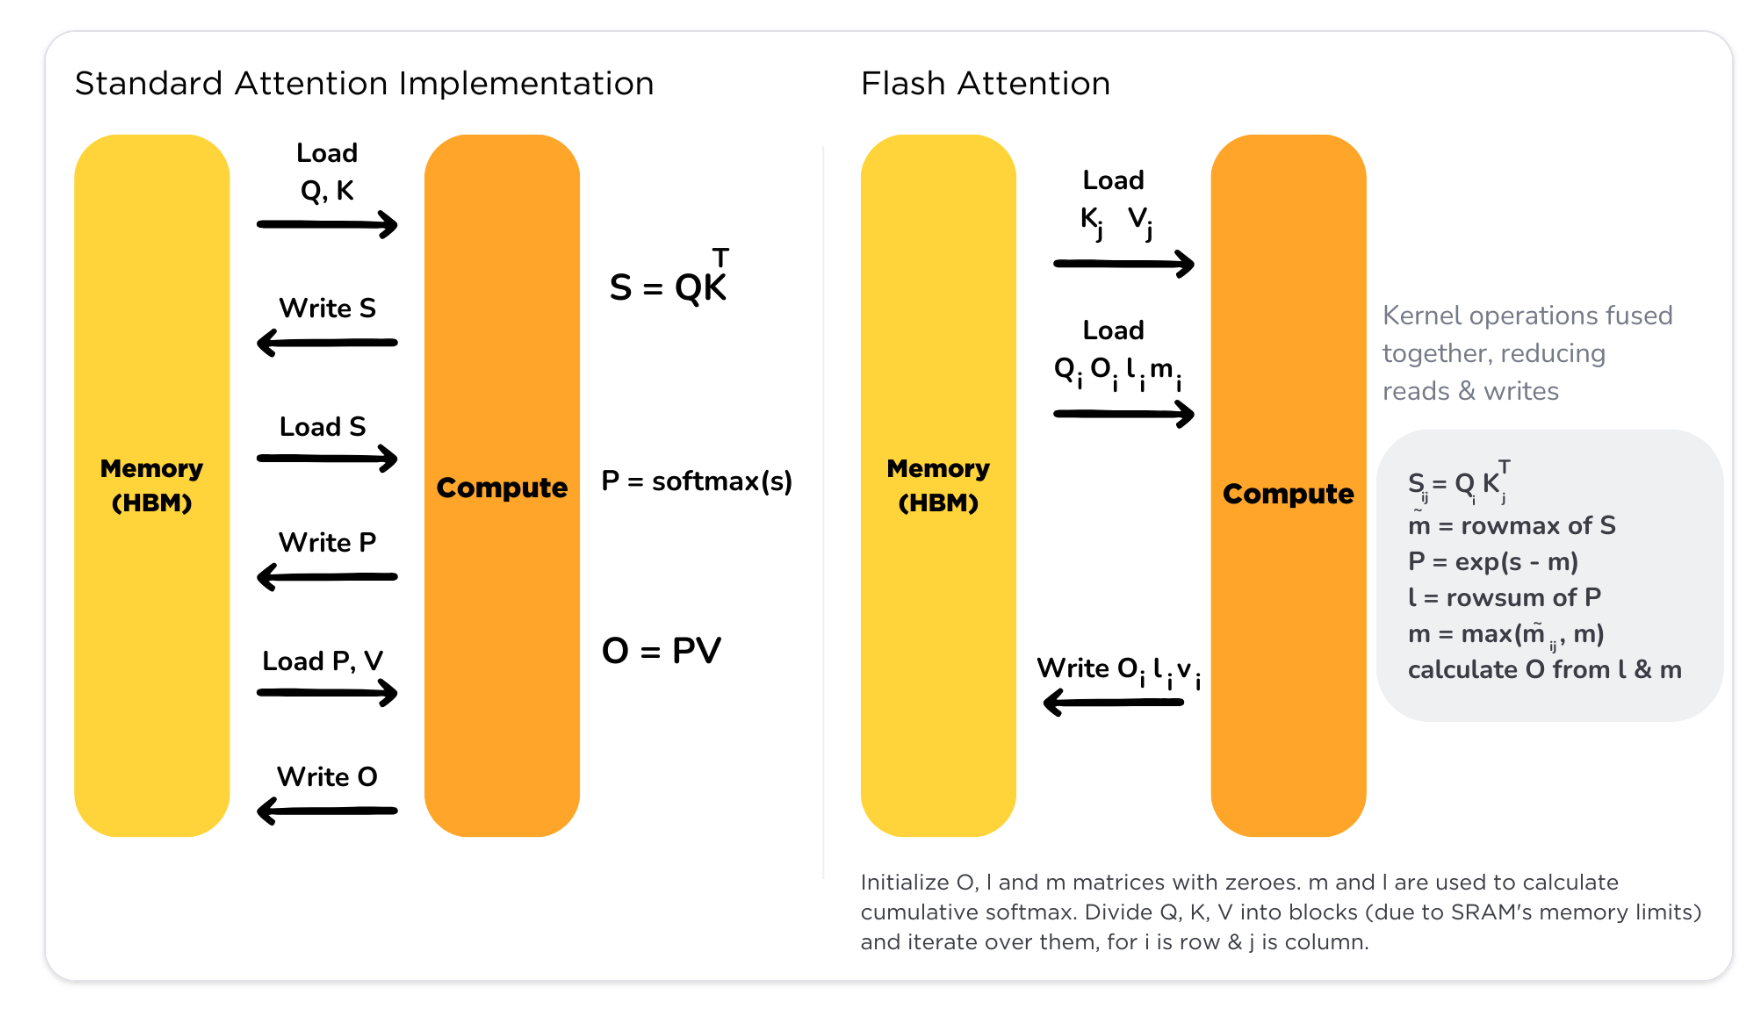
\includegraphics[width=0.6\textwidth]{figures/flash-attention}\\
                    \end{figure}
            \end{itemize}
    \end{itemize}
\end{frame}

\section{Efficient finetuning}

\begin{frame}
    {Improve finetuning efficiency}

    Problem:\\
    \begin{itemize}
        \item In NLP, typically all parameters of the pretrained models (e.g., BERT) are finetuned, which is expensive for large models.
        \item Saving and loading finetuned models for different tasks is costly.
    \end{itemize}
    \pause

    Can we finetune a smaller number of parameters to achieve performance similar to full finetuning?\\\pause
    \begin{itemize}
        \item Select a subset of parameters from the pretrained weights to update 
        \item Add a small number of parameters to adapte the (frozen) pretrained model
    \end{itemize}
\end{frame}

\begin{frame}
    {Finetune a subset of parameters}

    Freezing the first X layers \href{https://arxiv.org/pdf/1911.03090.pdf}{[Lee et al., 2019]} \\[1ex]

    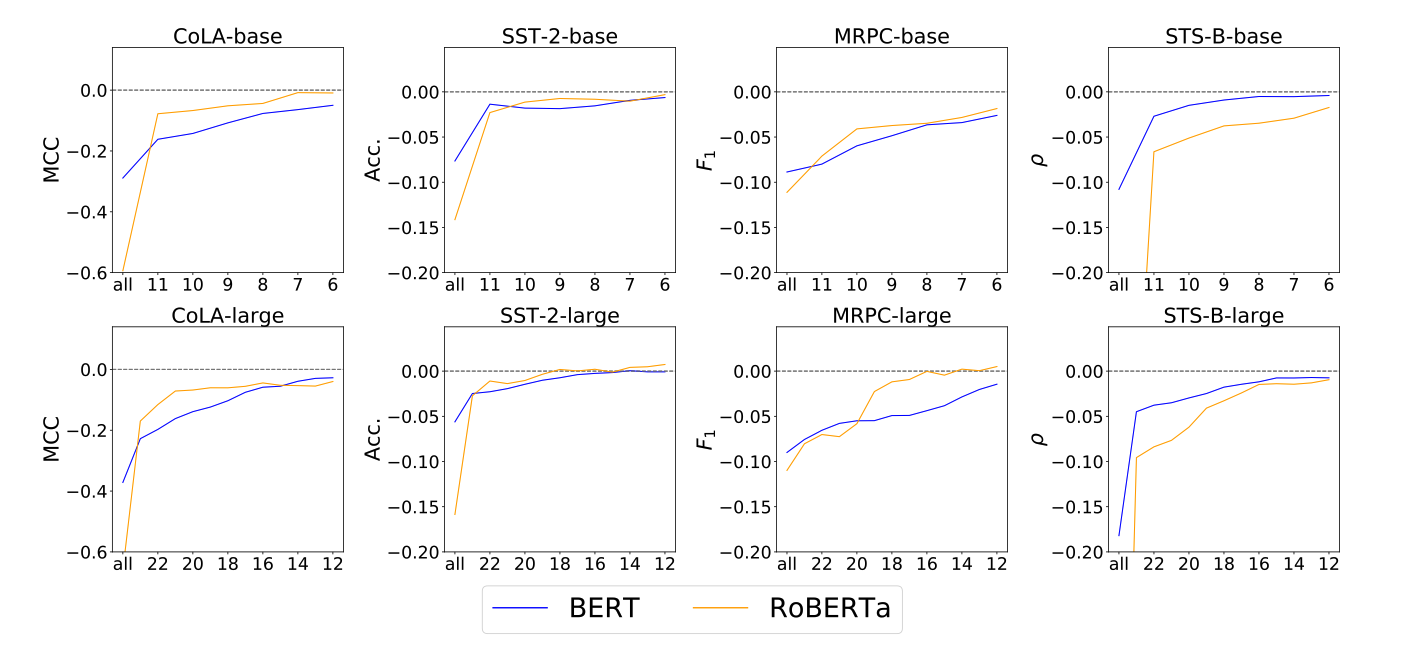
\includegraphics[width=\textwidth]{figures/layer-freezing}\\

    A fourth of the layers need to be fine-tuned to obtain 90\% of the performance.
\end{frame}

\begin{frame}
    {Finetune a subset of parameters}

    \textbf{BitFit} \href{https://arxiv.org/pdf/2106.10199.pdf}{[Ben-Zaken et al., 2022]}: only finetune the bias term (\blue{0.1\%} of the parameters) \\[1em]

    \begin{tikzpicture}
        \node (a) {Bias terms in QKV projection};
        \node (a-img) [below=0cm of a] {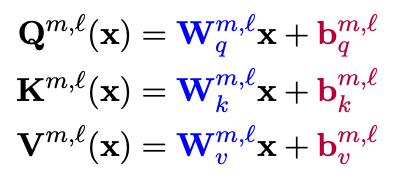
\includegraphics[height=3cm]{figures/bias-1}};
        \node (b-img) [right= of a-img] {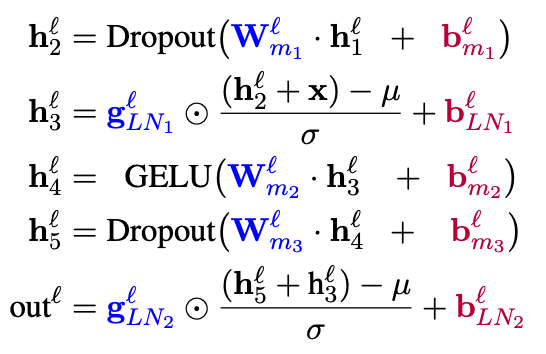
\includegraphics[height=3cm]{figures/bias-2}};
        \node (b) [above=0cm of b-img]{Bias terms in MLP layers};
    \end{tikzpicture}

    \medskip
    Result: 80.9 (BitFit, 0.08\% params) vs 81.8 (full finetuning) on GLUE
\end{frame}

\begin{frame}
    {Adapt the frozen pretrained model}

    \textbf{Adapter} \href{https://arxiv.org/pdf/1902.00751.pdf}{[Houlsby et al., 2019]}: insert small networks to the pretrained model \\[1em]

    \begin{columns}
        \begin{column}{0.4\textwidth}
    \begin{figure}
        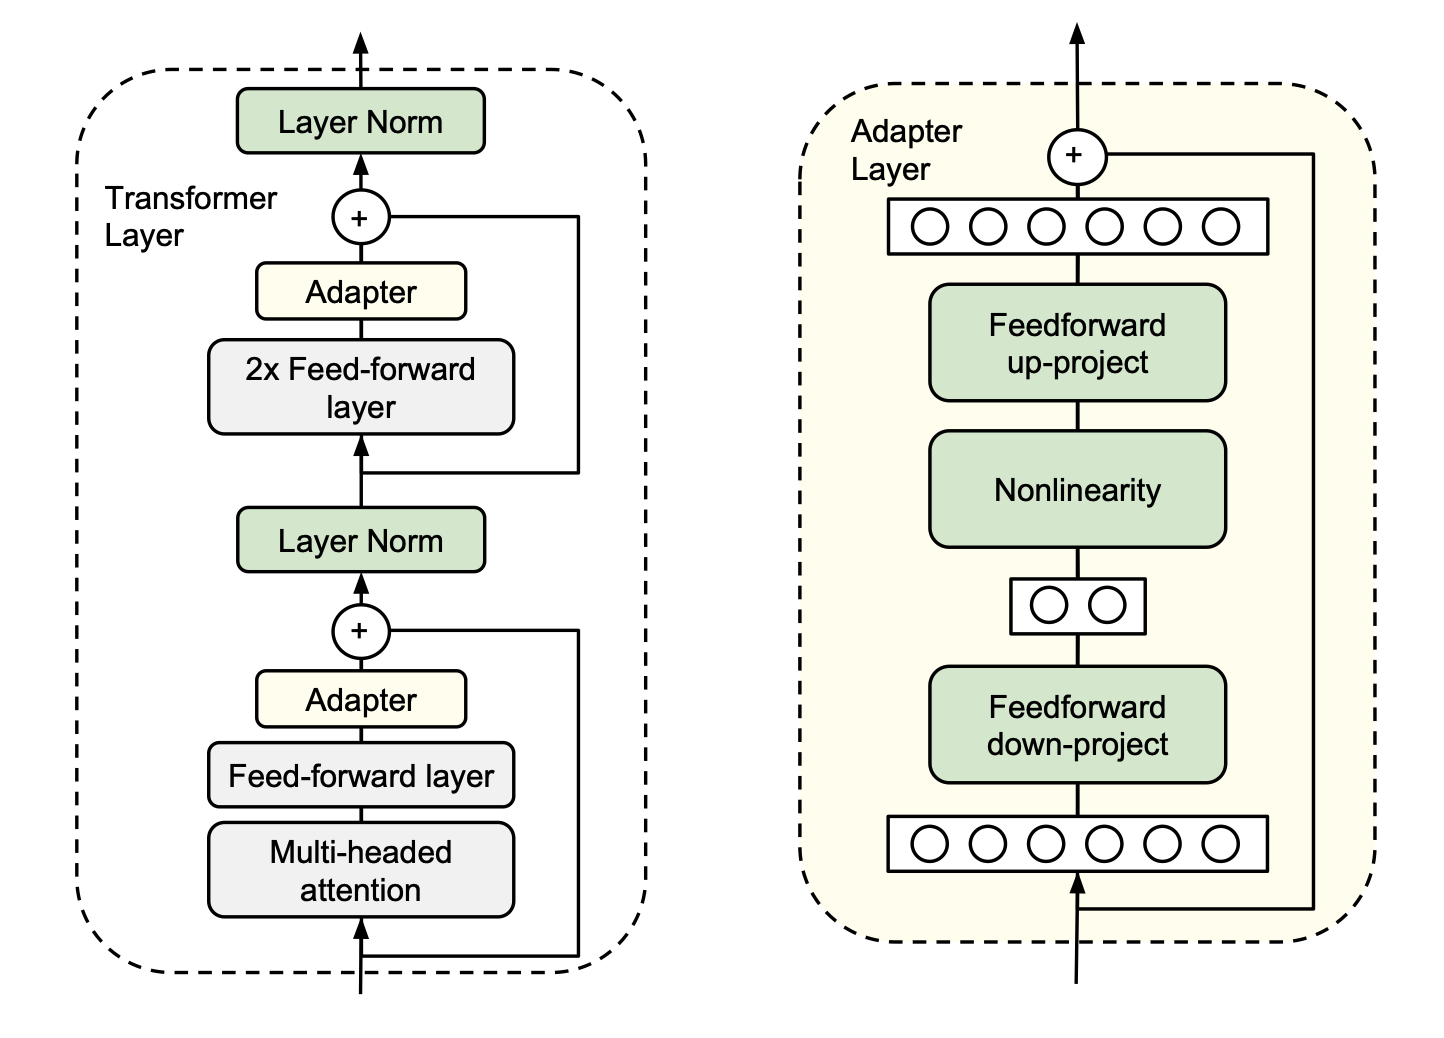
\includegraphics[width=\textwidth]{figures/adapter}
    \end{figure}
    \end{column}
        \begin{column}{0.6\textwidth}
            \begin{itemize}
                \item Insert learnable "adapters" in-between layers
                \item Adapters uses a \blue{bottleneck} structure to reduce parameters
                \item Adapters uses a \blue{skip-connection} \pause such that it can be ``reduced'' to the original frozen model
            \end{itemize}
            Result: less than 0.4\% performance drop with 3\% more parameters on GLUE
        \end{column}
    \end{columns}
\end{frame}

\begin{frame}
    {Adapt the frozen pretrained model}

    \textbf{LoRA} \href{https://arxiv.org/pdf/2106.09685.pdf}{[Hu et al., 2021]}: add low-rank matrices as additional parameters  \\\bigskip

    \begin{columns}
        \begin{column}{0.3\textwidth}
    \begin{figure}
        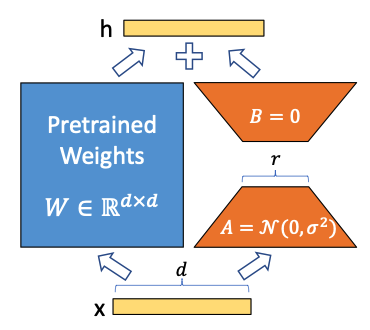
\includegraphics[width=\textwidth]{figures/lora}
    \end{figure}
    \end{column}
        \begin{column}{0.7\textwidth}

            \textbf{Hypothesis}: weight matrices are low rank
            \medskip

            \blue{Adapters}: For any matrix multiplication $h=W_0x$, we modify it to
            $$
            h = W_0x + \blue{\Delta W}x = W_0x + \blue{BA}x
            $$

            \begin{itemize}
                \item $W_0\in\BR^{d\times k}, B\in \BR^{d\times r}, A\in \BR^{r\times k} (r \ll k)$
                \item Initialization: $BA=0$
                \item Can be applied to any weight matrices, e.g., QKV projection matrices
            \end{itemize}
        \end{column}
    \end{columns}
\end{frame}

\begin{frame}
    {Adapt the frozen pretrained model}

    Compare LoRA and the original adapters:
    \begin{itemize}
        \item LoRA \blue{recovers full finetuning} by increasing $r$
        \item[] Adapter recovers an MLP model with increasing params
            \pause
        \item LoRA has \blue{no additional inference cost}
            \pause by setting $W_0 \leftarrow W_0 + BA$ (doesn't work for multiple tasks)
        \item[] Adapter incurs additional inference cost due to the added params
    \end{itemize}

    The most widely used efficient finetuning method on very large models ($>$100B).
\end{frame}

\begin{frame}
    {Summary}

    Reduce finetuning cost by reducing the number of parameters to update\\
    \begin{itemize}
        \item Finetune a subset of parameters
        \item Finetune an additional adapters inserted to the model
        \item System approach: mixed-precision training (e.g., converting some or all params to fp16)
    \end{itemize}

    %Not widely used for SOTA large models, but used sometimes in resource-constrained settings.

    Other ways to adapt the model without parameter update: prompting, in-context learning (later)

    %Lots of open research questions!

\end{frame}

\end{document}
